Prvi model za detekciju objekata zasnovan na konvolucijskim mrežama koji ćemo opisati je Regions with CNN features ili R-CNN (\cite{DBLP:journals/corr/GirshickDDM13}). Na skupu podataka VOC2012 je postigao 30\% veću prosječnu preciznost od prethodno najboljih modela. 
R-CNN sustav za detekciju objekata se sastoji od tri dijela. Detekcija R-CNN modelom ilustrirana je na slici \ref{rcnn}. Prvi dio generira prijedloge regija u kojima bi se mogao nalaziti objekt. Za predlaganje regija se može koristiti bilo koja metoda, ali autori koriste selektivnu pretragu kojom generiraju oko 2000 regija za svaku sliku.
Nakon toga se svaka regija šalje u drugi dio modela, duboku konvolucijsku mrežu, koja na izlazu daje 4096-dimenzionalni vektor dubokih značajki. Arhitektura mreže nije strogo definirana pa se može izabrati proizvoljno, ali izbor arhitekture u velikoj mjeri utječe na performanse modela. Konvolucijska mreža na ulazu očekuje RGB sliku dimenzija $227 \times 227$ u kojoj je vrijednostima piksela oduzeta srednja vrijednost piksela. Budući da su regije proizvoljnih veličina, prije prosljeđivanja regije konvolucijskoj mreži, mijenjaju joj se dimenzije na $227 \times 227$ bez obzira na omjer visine i širine. Prije mijenjanja dimenzija regije, prozor koji određuje regiju se proširuje za 16 piksela sa svake strane.
Treći dio modela čine binarni klasifikatori koji klasificiraju vektor dubokih značajki u neki od razreda. Za svaki razred se trenira jedan SVM koji označava regiju kao pozitivnu ili negativnu. Ako svi klasifikatori označe regiju kao negativnu, regija se smatra pozadinom.
Na kraju se svaka detekcija dovodi na ulaz jednostavnom modelu koji za predloženu regiju predviđa konačni prozor u kojem se nalazi objekt kako bi se poboljšala točnost detekcije.
Svaka komponenta modela se trenira posebno. Skup podataka za trening sastoji se od slika, regija predloženih selektivnom pretragom i konačnih detekcija s klasama objekata.
Konvolucijska mreža se predtrenira na skupu podataka za klasifikaciju slika, a zatim se trening nastavlja za klasifikaciju predloženih regija. Ako je omjer presjeka i unije predložene regije i stvarnog prozora u kojem se nalazi objekt veći od određenog praga (npr. 0.3), regija se klasificira kao da sadrži objekt, inače se klasificira kao pozadina.
Nakon treninga konvolucijske mreže, treniraju se klasifikatori (SVM), po jedan za svaki razred. Za trening klasifikatora se koriste duboke značajke dobivene iz regije konvolucijskom mrežom. Razredi regija se određuju na isti način kao i kod treninga konvolucijske mreže.
Modeli koji predviđaju konačne koordinate prozora se treniraju posebno za svaki razred. Za njihov trening se koriste predviđene regije kao ulazni podaci i stvarne lokacije objekata kao očekivani izlazi.

 \begin{figure}
	\centering
	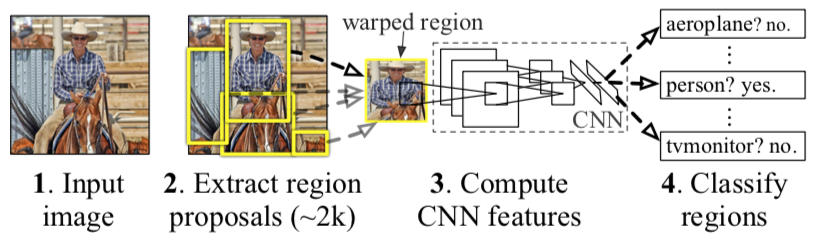
\includegraphics[scale=1]{img/rcnn.png}
	\caption{Vizualizacija detekcije R-CNN modelom.}
	\label{rcnn}
\end{figure}

